\documentclass{beamer}
\beamertemplatenavigationsymbolsempty

\title[Asian Englishes]{Asian Englishes\\ World Englishes}
\author[Francis Bond]{Francis Bond}
\date{2025}



\usepackage{tikz}
\usepackage{graphicx}
\usepackage{fontspec}
\usepackage{xeCJK}
\setCJKmainfont{Noto Sans CJK SC}
\newfontfamily\Libertine[Mapping=tex-text]{Linux Libertine O}
\usetheme{Madrid}
\usecolortheme{crane}

\usepackage{mygb4e}
\renewcommand{\eachwordtwo}{\Libertine}
\usepackage[e]{mtg2e}
\usepackage{xcolor}
\renewcommand{\mtcitestyle}[1]{\textcolor{teal}{\textit{#1}}}
\newcommand{\msa}{\mtciteform}
\newcommand{\lex}[1]{\textbf{\mtcitestyle{#1}}}
\usepackage[round]{natbib}

\begin{document}

% Title Slide
\begin{frame}
    \titlepage
\end{frame}

% (1) Overview / roadmap slide
\begin{frame}{Overview}
  \tableofcontents
\end{frame}


\section{World Englishes}


% Slide 1: What Are World Englishes?
\begin{frame}{What Are World Englishes?}
\textbf{Definition:}
\begin{itemize}
    \item The global varieties of English spoken in diverse cultural, social, and linguistic contexts.
    \item Includes \textbf{Inner Circle}, \textbf{Outer Circle}, and \textbf{Expanding Circle} Englishes \citep{Kachru:1985}.
\end{itemize}

\textbf{Importance:}
\begin{itemize}
    \item Reflects the spread of English as a global lingua franca.
    \item Highlights the adaptability and localization of English in different regions, especially in Asia.
\end{itemize}

\textbf{Examples:}
\begin{itemize}
    \item British English, Indian English, Chinese English, Nigerian English.
\end{itemize}
\end{frame}


% Slide 4: Kachru's Three Circles
\begin{frame}{Kachru's Three Circles of English}
\centering
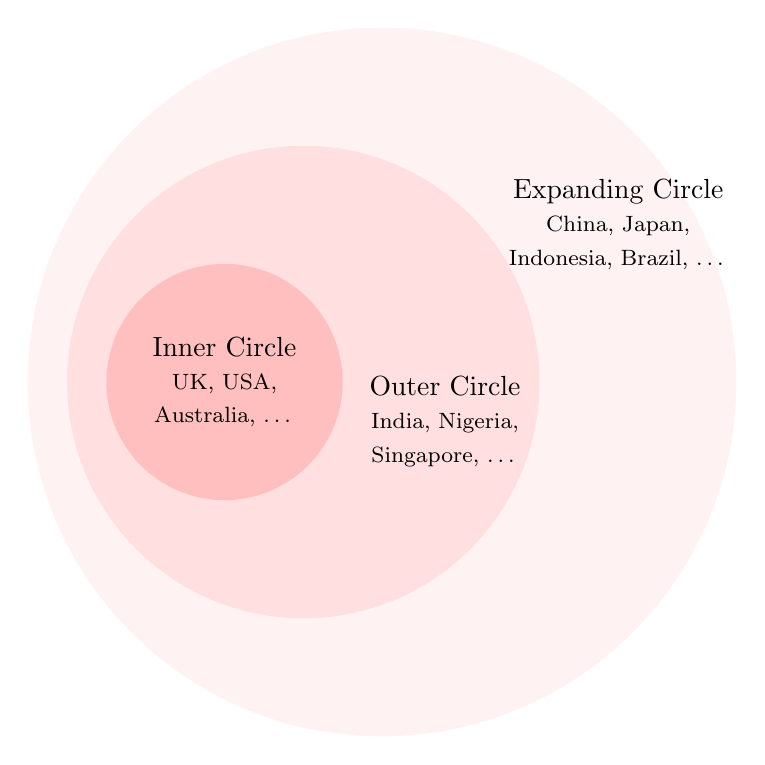
\begin{tikzpicture}

    % Expanding Circle
    \fill[fill=pink!20] (0,0) circle [radius=4.5];

    % Outer Circle
    \fill[fill=pink!50] (-1,0) circle [radius=3];
    \node[align=center] at (.8,-.5) {Outer Circle \\
      \footnotesize India, Nigeria, \\  \footnotesize Singapore, \ldots};

   % Inner Circle
  \fill[fill=pink] (-2,0) circle [radius=1.5];
  \node[align=center] at (-2,0) {Inner Circle\\
    \footnotesize UK, USA, \\  \footnotesize  Australia, \ldots};

  \node[align=center] at (3, 2) {Expanding Circle \\ \footnotesize China, Japan,  \\ \footnotesize Indonesia, Brazil, \ldots};

\end{tikzpicture}

\bigskip
\begin{center}
  \small After \citet{Kachru:1985}: Inner, Outer and Expanding Circles of English.
\end{center}
\end{frame}


\begin{frame}{The Inner Circle}
\textbf{Definition:}
\begin{itemize}
    \item Represents countries where English is the native language and primary means of communication.
\end{itemize}

\textbf{Examples:}
\begin{itemize}
    \item United Kingdom, United States, Australia, Canada, New Zealand.
\end{itemize}

\textbf{Key Features:}
\begin{itemize}
    \item  England and former settler colonies where English became dominant (USA, Canada, Australia, New Zealand).
    \item Sets linguistic norms often viewed as "standard" English.
    \item Used as a cultural identifier.
\end{itemize}

\end{frame}

% Slide 2: Outer Circle
\begin{frame}{The Outer Circle}
\textbf{Definition:}
\begin{itemize}
    \item Countries where English serves as a second language, often used in government, education, and business.
    \item Reflects historical colonial influence.
\end{itemize}

\textbf{Examples:}
\begin{itemize}
\item India, Nigeria, Singapore, Philippines.
\item Singapore fits almost all characteristics of inner circle  except origin, \ldots
\end{itemize}

\textbf{Key Features:}
\begin{itemize}
    \item Nativized varieties of English.
    \item High degree of multilingualism among speakers.
    \item Functional roles in administration and education.
    \item More speakers than the inner circle
\end{itemize}

\end{frame}

% Slide 3: Expanding Circle
\begin{frame}{The Expanding Circle}
\textbf{Definition:}
\begin{itemize}
    \item Countries where English is used as a foreign language.
    \item Primarily for international communication and business.
\end{itemize}

\textbf{Examples:}
\begin{itemize}
    \item China, Japan, Brazil, Russia.
\end{itemize}

\textbf{Key Features:}
\begin{itemize}
    \item Does not have a colonial legacy of English.
    \item Lacks institutionalized functions in government or education.
    \item Growing role in globalization and digital communication.
    \item Has the most speakers!
\end{itemize}

\end{frame}

\begin{frame}{English-speaking populations across various countries.}
  \begin{center}
\small
\begin{tabular}{lrrrrrrr}
  \textbf{Country} & \textbf{ Population} & \textbf{Speakers }  & \textbf{First L}  & \textbf{Other L}  \\ \hline
United States & 312,092,668 & 297,400,000 & 244,232,103 & 42,155,719 \\ 
India & 1,450,000,000 & 228,539,090 & 259,678 & 228,279,412 \\ 
Nigeria & 206,200,000 & 125,039,680 & 20,000,000 & 103,198,040  \\ 
Pakistan & 220,892,331 & 108,044,691 & 8,642 & 108,036,049  \\ 
United Kingdom & 64,000,000 & 62,912,000 & 59,072,000 & 3,840,000 \\ 
Philippines & 110,000,000 & 70,117,935 & 36,935 & 70,081,000  \\ 
Germany & 80,600,000 & 45,400,000 & 392,000 & 45,100,000  \\ 
Uganda & 44,270,000 & 19,800,000 & 0 & 19,800,000  \\ 
France & 67,500,000 & 38,643,750 & 0 & 38,643,750  \\ 
Canada & 37,138,500 & 30,480,750 & 20,193,335 & 10,287,415  \\ 
Egypt & 110,990,000 & 44,373,802 & 5,527,302 & 38,846,500  \\ 
Australia & 23,401,892 & 21,715,910 & 17,020,421 & 4,695,489  \\ 
Bangladesh & 165,323,100 & 19,838,772 & 709,873 & 16,398,158 \\ 
Poland & 38,501,000 & 18,890,000 & 103,541 & 18,786,459  \\ 
Ghana & 27,000,000 & 18,000,000 & 0 & 18,000,000  \\[1ex] 
Singapore & 4,044,200 & 3,900,000 & 1,953,348 & 1,946,652 
\end{tabular}
    
\end{center}
{\footnotesize Data from  \href{https://en.wikipedia.org/wiki/List_of_countries_by_English-speaking_population}{Wikipedia: List of countries by English-speaking population}.\\
\textbf{Takeaway:} There are more English speakers in India than in any single ``Inner Circle'' country.}
\end{frame}

% Slide 1: General Debate
\begin{frame}{World Englishes: Quirk vs. Kachru}
\textbf{Quirk's Perspective (Uniformity View, \citeyear{Quirk:1985we}):}
\begin{itemize}
    \item Emphasizes a single, standardized form of English based on Inner Circle norms (e.g., UK, US).
    \item Concerns about intelligibility and global communication.
    \item Argues that legitimizing non-standard varieties risks misunderstanding.
      \\ \emph{We need one standard English for effective international communication}
  \end{itemize}

\textbf{Kachru's Perspective (Pluralist View, \citeyear{Kachru:1985}:}
\begin{itemize}
    \item Advocates for the legitimacy of Outer Circle varieties (e.g., Indian, Nigerian English).
    \item Emphasizes linguistic and cultural adaptation (nativization).
    \item Critiques the deficit model of "errors" and promotes ownership of English by all its users.
      \emph{English belongs to all its users, not just its historical 'native' speakers.}
    \end{itemize}
  \end{frame}

% Slide 2: Key Themes of the Debate
\begin{frame}{Key Themes of the Debate}
\begin{itemize}
    \item \textbf{Standardization vs. Diversity:}
    \begin{itemize}
        \item Quirk: Standardization is essential for global intelligibility.
        \item Kachru: Diversity reflects the realities of English use worldwide.
    \end{itemize}
    \item \textbf{Pedagogical Implications:}
    \begin{itemize}
        \item Quirk: Teaching should adhere to Inner Circle norms.
        \item Kachru: Teaching should validate localized varieties.
    \end{itemize}
    \item \textbf{Ownership of English:}
    \begin{itemize}
        \item Quirk: English belongs to the Inner Circle.
        \item Kachru: English is the global property of all its users.
    \end{itemize}
\end{itemize}
\end{frame}

% Slide 3: Kachru's Four False Assumptions
\begin{frame}{Four ``False Assumptions'' about English \citep{Kachru:1992}}
\textbf{1. The Homogeneity Assumption:}
\begin{itemize}
    \item \textbf{Assumption:} There is a single, homogeneous standard English.
    \item \textbf{Counterpoint:} Inner Circle varieties themselves exhibit variation.
\end{itemize}

\textbf{2. The Deficit Model of Non-Native Varieties:}
\begin{itemize}
    \item \textbf{Assumption:} Outer Circle Englishes are "deviant" or deficient.
    \item \textbf{Counterpoint:} Outer Circle varieties are contextually legitimate adaptations.
\end{itemize}

\textbf{3. The Pedagogical Purity Assumption:}
\begin{itemize}
    \item \textbf{Assumption:} Teaching should focus on Inner Circle norms exclusively.
    \item \textbf{Counterpoint:} Teaching should reflect local linguistic realities.
\end{itemize}

\textbf{4. The Intelligibility Assumption:}
\begin{itemize}
    \item \textbf{Assumption:} Inner Circle norms guarantee mutual intelligibility.
    \item \textbf{Counterpoint:} Intelligibility is context-dependent and mutual.
\end{itemize}
\end{frame}



% Slide B4: Innovation – Deviation – Mistake
\begin{frame}{Innovation\ –\  Deviation\ –\  Mistake (Kachru, 1992)}
\textbf{Key Distinctions:}
\begin{itemize}
    \item \textbf{Innovation:} Creativity in language use; often denied to Outer and Expanding Circle speakers.\\
      \emph{Examples:} \eng{timepass}, \eng{skinship}, \eng{add oil}.
    \item \textbf{Deviation:} Comparison with another variety; implies departure from a norm.\\
      \emph{Example (vs. Inner Circle norm):} \eng{He is knowing the answer.}
    \item \textbf{Mistake (or error):} Related to acquisitional deficiency; not accepted in any stable speech community.\\
      \emph{Example:} \eng{He knowed the answer.}
\end{itemize}

Different varieties are held to different standards!
    
\end{frame}


% Slide B5: Standards Across Space
\begin{frame}{Standards Across Space}
\textbf{Three often-cited ``standard'' varieties:}
\begin{itemize}
    \item British English (BrE), North American English (especially AmE), and Australian English (AusE).
    \item Similarities and differences:
    \begin{itemize}
        \item Across the three standards.
        \item Across varieties within each region (e.g., different UK or US dialects).
    \end{itemize}
    \item Pronunciation
    \item Vocabulary: The Most Noticeable Divergence (NAmE vs. BrE)
    \begin{itemize}
        \item \textbf{Extended meanings:} e.g., \eng{corn, robin}.
        \item \textbf{New words:} e.g., \eng{buttle} ``to act as a butler''.
        \item \textbf{Borrowings:} e.g., \eng{moccasin, squash, toboggan}.
    \end{itemize}
    \item Since US independence:
    \begin{itemize}
        \item Technological terms: e.g., \eng{windshield} vs. \eng{windscreen}.
    \end{itemize}
\end{itemize}
\end{frame}


% Slide B5: Australian English
\begin{frame}{Australian English}
\textbf{Key Features:}
\begin{itemize}
    \item Borrowings from Aboriginal languages: e.g., \eng{kangaroo, boomerang}.
    \item Unique slang words and phrases.
    \item Common use of abbreviations and clippings.
      \\ \eng[bbq]{barbie}, \eng[university]{uni}, \eng[sandwich]{sanger}, \eng[relative]{relly}, \eng[make a U-turn]{chuck a U-ey}
      \\ \eng[person with white hair]{Snowy}, \eng[red-head]{Bluey}, \eng[Bond (me)]{Bondie}
\end{itemize}
\end{frame}

% Slide B5: Grammar Differences
\begin{frame}{Quite a lot of Grammar Differences}
\textbf{AmE vs. BrE \citep{Trudgill:Hannah:2002}:}
\begin{itemize}
    \item \textbf{Verbs:} Morphology, auxiliaries.
    \begin{itemize}
        \item US: \eng{He did already eat.} vs. UK: \eng{He has already eaten.}
    \end{itemize}
    \item \textbf{Nouns:} Endings, use of verbs as nouns.
    \begin{itemize}
        \item US: \eng{Please action this.} vs. UK: \eng{Please do this/act on this.}
    \end{itemize}
    \item \textbf{Adjectives and Adverbs:}
    \begin{itemize}
    \item US: \eng{He runs real fast.} vs. UK: \eng{He runs really fast.}
    \item US: \eng{How big of a room is it?} vs. UK: \eng{How big a room is it?}
    \end{itemize}
    \item \textbf{Prepositions:}
    \begin{itemize}
        \item US: \eng{I went on the weekend.} vs. UK: \eng{I went at the weekend.}
    \end{itemize}
\end{itemize}
\end{frame}

% Slide B6: Native and Non-Native Speakers
\begin{frame}{Native and Non-Native Speakers of English}
\textbf{Criticisms of NS/NNS Terms:}
\begin{itemize}
    \item NS = \textit{native speaker}, NNS = \textit{non-native speaker} (apparently simple labels, but problematic).
    \item Assumes monolingualism is the norm.
    \item Overemphasizes order of acquisition.
    \item Reinforces Anglo speakers as reference points.
    \item Implies unidirectional power relationships.
    \item Encourages simplistic views of "errors."
    \item What do these labels suggest about \emph{you} as speakers of English?
\end{itemize}
\end{frame}

% Slide B6: Alternatives to NS/NNS
\begin{frame}{Alternatives to NS/NNS Distinction}
\textbf{\citet{Rampton:1990}: "Experts" $\rightarrow$ Expertise}
\begin{itemize}
    \item Advantages:
    \begin{itemize}
        \item Learned, not innate.
        \item Relative, partial, and contestable.
    \end{itemize}
        \item Disadvantages:
    \begin{itemize}
        \item "Non-expert" implies value judgment.
    \end{itemize}
\end{itemize}

\textbf{\citet{Jenkins:2000}: MES, BES, NBES}
\begin{itemize}
    \item MES: Monolingual English Speaker.
    \item BES: Bilingual English Speaker.
    \item NBES: Non-Bilingual English Speaker.
    \item Emphasizes speakers' bilingual repertoires rather than a simple native vs. non-native divide.
\end{itemize}
\end{frame}

\begin{frame}{Naming the Varieties: Labels and Ideology}
\small
\textbf{Names are not neutral:} they index attitudes, power, and ownership.
\medskip

\begin{itemize}
  \item \textbf{Indian English}: \eng{Hinglish}  \\
    \eng{Hinglish} highlights code-mixing and youth / pop-culture identities, but can also stereotype.

  \medskip
  \item \textbf{Singapore \& Malaysian English}: \eng{Singlish} / \eng{Manglish} \\
    In official discourse we often find \textit{Colloquial Singapore English} (CSE).\\
    Government campaigns (\emph{Speak Good English}) frame \eng{Singlish} as a problem, while speakers use the name to index solidarity and local identity.

  \medskip
  \item \textbf{Hong Kong English}:  \eng{Chinglish}  \\
    Labels like \eng{Chinglish} are common in media but are usually mocking or deficit-oriented, focusing on ``errors'' in signs or speech.

  \medskip
  \item \textbf{Japanese English, wasei-eigo}: \eng{Japlish}, \eng{Engrish}   \\
    \textit{Japanese English} and \textit{wasei-eigo} are descriptive terms used in linguistics.\\
    Informal labels like \eng{Engrish} or \eng{Japlish} are often used from outside Japan and carry racist / mocking connotations.
\end{itemize}
\end{frame}


% (3) Activity slide for NS/NNS / labels
\begin{frame}{Activity: How Would You Label Yourselves?}
\small
\begin{itemize}
  \item In small groups, discuss which labels you prefer:
  \begin{itemize}
    \item NS / NNS
    \item MES / BES / NBES
    \item Something else entirely?
  \end{itemize}
  \item How do these labels affect:
  \begin{itemize}
    \item how confident you feel when speaking English?
    \item how you evaluate other people’s English?
    \end{itemize}
  \item  Who gets to name a variety (state, teachers, speakers, outsiders)?\\
    How do different labels affect the \emph{prestige} and \emph{legitimacy} of these Englishes?
  \end{itemize}

% \medskip
% \textbf{Would you change the terminology in English teaching at Palacký? Why / why not?}
\end{frame}



% Slide B7: Codification of Asian Englishes
\begin{frame}{En Route to New Standard Englishes}
\textbf{Codification of Asian Englishes:}
\begin{itemize}
    \item Importance:
    \begin{itemize}
        \item Acceptance, prestige, classroom model.
    \end{itemize}
    \item Obstacles:
    \begin{itemize}
        \item Indigenized varieties seen as "interlanguages."
        \item SLA perspective emphasizes NS-like competence.
        \item Motivation for acquisition is integrative (admiration for NS culture).
    \end{itemize}
\end{itemize}
\end{frame}



% Slide 3: Characteristics of Asian Englishes
\begin{frame}{Characteristics of Asian Englishes}
\textbf{Distinct Features:}
\begin{itemize}
    \item \textbf{Phonology:} Unique accents and stress patterns (e.g., Indian English retroflex sounds).
    \item \textbf{Syntax:} Influence of local languages (e.g., omission of articles in Singapore English).
    \item \textbf{Lexicon:} Borrowings and cultural terms (e.g., \eng[seal/stamp]{chop} in Malaysian English).
    \item Extensive code-switching
\end{itemize}
\end{frame}

\section{Indian English}

\begin{frame}
\frametitle{What is Indian English?}
\begin{itemize}
    \item Indian English refers to the variety of English spoken in India.
    \item It is influenced by India's multilingual environment and local languages.
    \item Features unique vocabulary, pronunciation, grammar, and idiomatic expressions.
    \item Recognized as one of the most widespread second languages in India.
\end{itemize}
\end{frame}

\begin{frame}
\frametitle{Key Features of Indian English}
\begin{itemize}
    \item \textbf{Pronunciation:}
    \begin{itemize}
        \item Often rhotic: Pronouncing /r/ in words like \eng{car} and \eng{farm.}
        \item Vowel quality may differ from US/UK norms (e.g., \eng{bat}, \eng{bad}, \eng{bed}).
    \end{itemize}
    \item \textbf{Vocabulary:}
    \begin{itemize}
        \item Unique words like \eng{prepone} (to reschedule earlier) and \eng{godown} (warehouse).
    \end{itemize}
    \item \textbf{Grammar:}
    \begin{itemize}
        \item Use of the progressive tense: \eng{He is knowing the answer.}
        \item Use of \eng{doubt} in the sense of ``question'': \eng{He is having a doubt in mathematics.}
    \end{itemize}
\end{itemize}
\end{frame}

\begin{frame}
\frametitle{Unique Vocabulary in Indian English}
\begin{itemize}
    \item \textbf{Borrowed words:}
    \begin{itemize}
        \item \eng{bungalow} (from Hindi: "bangla")
        \item \eng{jungle} (from Hindi: "jangal")
    \end{itemize}
    \item \textbf{Hybrid expressions:}
    \begin{itemize}
        \item \eng{pass out} (to graduate)
        \item \eng{out of station} (not in town)
    \end{itemize}
    \item \textbf{Local adaptations:}
    \begin{itemize}
        \item \eng{hill station} (mountain resort)
        \item \eng{timepass} (leisure activity)
        \item \eng{revert} (reply --- also used in Manglish/Singlish)
    \end{itemize}
\end{itemize}
\end{frame}

\begin{frame}
\frametitle{Examples of Indian English Sentences}
\begin{itemize}
    \item \eng{Can you prepone the meeting to tomorrow?}
    \item \eng{I passed out of college in 2020.}
    \item \eng{He is having a doubt in mathematics.}
    \item \eng{She went to the market to buy vegetables only.}
    \item \eng{Let us go for a walk in the evening, no?}
\end{itemize}
\end{frame}

\begin{frame}
\frametitle{Cultural and Linguistic Significance}
\begin{itemize}
    \item Indian English reflects the diversity of India's languages and cultures.
    \item It bridges communication gaps in a multilingual society.
    \item Used in government, education, business, and media.
    \item Contributes to the global spread of English with a distinct identity.
\end{itemize}
\end{frame}


\section{Singlish (Manglish)}


\begin{frame}
\frametitle{What is Singlish?}
\begin{itemize}
    \item Singlish is the colloquial form of English spoken in Singapore.
    \item It combines English with elements from Malay, Tamil, Hokkien, Cantonese, and other languages.
    \item Singlish is informal and often spoken in casual settings.
    \item Although not officially endorsed, it is a key part of Singaporean identity.
\end{itemize}
\end{frame}


\begin{frame}
\frametitle{Examples of Singlish Vocabulary}
\begin{itemize}
\item \lex{Lah:} \eng{Don't worry lah!} (adds emphasis or assurance)
\item \lex{Kiasu:} \eng{He is so kiasu.} (fear of missing out)
\item \lex{Shiok:} \eng{This food is so shiok!} (delicious or enjoyable)
\item \lex{Blur:} \eng{Why are you so blur?} (confused or clueless)
\item \lex{Paiseh:} \eng{So paiseh to ask!} (embarrassed)
\item \lex{Ang moh:} \eng{The ang moh loves laksa.} (Caucasian - lit: red head)

\end{itemize}

\begin{center}
  Try our \href{https://singdict.github.io/}{Singlish Dictionary}!
\end{center}
\end{frame}

\begin{frame}
\frametitle{Singlish Grammar and Syntax}
\begin{itemize}
    \item \textbf{Aspect through adverbs, not tense:}
    \begin{itemize}
        \item \eng{He go already.} (He has already gone.)
    \end{itemize}
    \item \textbf{Tag particles:}
    \begin{itemize}
        \item \eng{You want coffee, ah?} (adds a questioning tone)
        \item \eng{Very expensive, leh.} (adds emphasis)
    \end{itemize}
    \item \textbf{Omission of articles/plurality:}
    \begin{itemize}
    \item \eng{I go market.} (I am going to the market.)
    \item \eng{I buy 3 book.} (I will buy three books.)
    \end{itemize}
\end{itemize}
\end{frame}

\begin{frame}
\frametitle{Cultural and Linguistic Significance}
\begin{itemize}
    \item Singlish reflects Singapore's multicultural heritage.
    \item It fosters a sense of local identity and camaraderie.
    \item Often used in media, humor, and casual conversations.
    \item Despite government efforts to promote Standard English, Singlish remains a vibrant and unique aspect of Singaporean culture.
\end{itemize}
\end{frame}


\section{Hong Kong English}



\begin{frame}
\frametitle{What is Hong Kong English?}
\begin{itemize}
    \item Hong Kong English is the variety of English influenced by Cantonese, the primary language spoken in Hong Kong.
    \item Developed due to British colonial rule (1842–1997) and remains significant in education, business, and law.
    \item Reflects a blend of British English, local linguistic features, and Cantonese cultural influence.
\end{itemize}
\end{frame}

\begin{frame}
\frametitle{Key Features of Hong Kong English}
\begin{itemize}
    \item \textbf{Pronunciation:}
    \begin{itemize}
        \item Influence of Cantonese tones on stress patterns.
        \item Some speakers may neutralize /r/ and /l/, producing similar sounds in words like \eng{rice} and \eng{lice}.
    \end{itemize}
    \item \textbf{Grammar:}
    \begin{itemize}
        \item Omission of articles and prepositions: \eng{I go market} (I am going to the market).
    \end{itemize}
    \item \textbf{Vocabulary:}
    \begin{itemize}
        \item Loanwords from Cantonese: \eng{yum cha} (drink tea) and \eng{char siu} (roast pork).
    \end{itemize}
\end{itemize}
\end{frame}

\begin{frame}
\frametitle{Examples of Hong Kong English Vocabulary}
\begin{itemize}
    \item \textbf{Loanwords from Cantonese:}
    \begin{itemize}
        \item \lex{Dai pai dong:} Open-air food stalls.
        \item \lex{Si fu:} Master or skilled worker.
        \item \lex{Cha chaan teng:} Hong Kong-style cafes.
    \end{itemize}
    \item \textbf{Hybrid expressions:}
    \begin{itemize}
        \item \lex{Add oil:} An encouragement or cheer, meaning \eng{keep going} or "good luck."
        \item \lex{Long time no see:} Often described as a calque from the Cantonese phrase "好耐冇見" (hou noi mou gin), though the exact origin is debated.
    \end{itemize}
\end{itemize}
\end{frame}

\begin{frame}
\frametitle{Common Features of Sentences in Hong Kong English}
\begin{itemize}
    \item \textbf{Direct translations from Cantonese:}
    \begin{itemize}
        \item \eng{He very smart, la.} (He is very smart, you know.)
    \end{itemize}
    \item \textbf{Different grammatical elements:}
    \begin{itemize}
        \item \eng{I no understand.} (I do not understand.)
    \end{itemize}
    \item \textbf{Unique phrases:}
    \begin{itemize}
        \item \eng{I go yum cha with family tomorrow.} (I am going to have dim sum with my family tomorrow.)
    \end{itemize}
\end{itemize}
\end{frame}

\begin{frame}
\frametitle{Cultural and Linguistic Significance}
\begin{itemize}
    \item Hong Kong English reflects the region's colonial past and its Cantonese-speaking majority.
    \item It plays a key role in education, government, and international business.
    \item Highlights the blending of British and Chinese cultures in Hong Kong.
    \item Despite its informal and localized nature, it remains an essential aspect of Hong Kong's identity and communication in multilingual settings.
\end{itemize}
\end{frame}


\section{Japanese English and Wasei-eigo}



\begin{frame}
\frametitle{What is Japanese English?}
\begin{itemize}
\item Japanese English refers to the variety of English influenced by the Japanese language.
  \begin{itemize}
  \item Informal labels like \eng{Japlish} or \eng{Engrish} are sometimes used for English produced by Japanese speakers, often in a mocking or racist way.
  \item 和製英語 \eng[Japanese-made English]{wasei eigo} are English-like words used in Japanese.
  \end{itemize}
    \item It often features adaptations of English words and phrases to fit Japanese phonetics and culture.
    \begin{itemize}
        \item Inserting vowels: \eng{table} becomes \eng{te-buru.}
        \item No distinction between /l/ and /r/: \eng{light} and \eng{right} sound similar.
        \item Fewer consonant clusters
        \item A tendency to shorten things
    \end{itemize}
    \item Developed due to English education, international business, and cultural exchange.
    \item Known for unique loanwords, katakana usage, and creative expressions.
    \end{itemize}

\end{frame}


\begin{frame}
\frametitle{Examples of Wasei Eigo}
\begin{itemize}
    \item \textbf{Adapted loanwords:}
    \begin{itemize}
    \item \lex{sarariman} (salaryman) ``male office worker''
    \item \lex{o-eru} (OL: office lady) ``female office worker''
        \item \lex{hando phon} (hand phone) ``Mobile phone (from \eng{handy phone})''
        \item \lex{baikingu} (viking) ``buffet'' (because Scandinavians like  \eng{smorgasbord})
    \end{itemize}
  \item \textbf{Creative coinages:}
      \begin{itemize}
      \item \lex{mai pe-su} (my pace) ``going at one's own speed''
      \item \lex{seku-hara}  ``sexual harassment''
        \item \lex{pauwa-hara} (power harassment) ``workplace bullying''
        \item \lex{konbini}  ``convenience store''
        \item \lex{sukinshippu} (skinship) ``physical closeness or bonding''
        \item \lex{ha-to furu} (heartfull) ``warm-hearted, caring''
    \end{itemize}
\end{itemize}
\end{frame}


\begin{frame}
\frametitle{Cultural and Linguistic Significance}
\begin{itemize}
    \item Japanese English showcases the cultural blending of Japan and the English-speaking world.
    \item Reflects creative adaptations to fit Japanese language structure and social norms.
    \item Plays an important role in education, tourism, and advertising in Japan.
    \item Despite challenges with pronunciation and syntax, it has become a unique and recognizable form of English globally.
\end{itemize}
\end{frame}


% Slide 5: The Future of Asian Englishes
\begin{frame}{The Future of Asian Englishes}
\textbf{Trends:}
\begin{itemize}
    \item Increasing prestige and global recognition.
    \item Growth of English as a second language in Asia.
    \item Integration into educational systems and digital platforms.
\end{itemize}

\textbf{Key Questions:}
\begin{itemize}
    \item How will globalization shape Asian Englishes?
    \item Will codification lead to the emergence of new standards?
    \item How can we balance intelligibility and diversity?
\end{itemize}
\end{frame}

\begin{frame}{Prestige and ``Non-Standard'' Varieties in the Inner Circle}

\begin{itemize}
  \item \textbf{Australian English} (\eng{Strine})  
    Historically stigmatized as ``broad'' or ``lazy'' English; now an accepted national standard.  \citep{Burridge:Mulder:1999}

  \item \textbf{African American Vernacular English (AAVE)} (\eng{ebonics})  
    A rule-governed, systematic variety with distinctive grammar (e.g.\ copula absence, habitual \eng{be}).  
    Frequently stigmatized despite high linguistic complexity and cultural prestige (music, media). \citep{Rickford:1999}

  \item \textbf{Appalachian / Southern US English}  
    Often mischaracterized as ``incorrect''; has unique grammatical systems (e.g.\ a-prefixing: \eng{He’s a-running}, multiple modals \eng{I shoulda coulda done it}).  
    Example of \textbf{overt vs.\ covert prestige}. \citep{LippiGreen:2012}

  \item \textbf{British regional dialects} (Scouse, Geordie, Glaswegian)  
    Local prestige but low institutional prestige; hard  for ousiders to understand.

\end{itemize}

\medskip
\textbf{Takeaway:} The ideology that Inner Circle Englishes are uniform ``standards'' is false: \emph{all Englishes exhibit prestige hierarchies}.
\end{frame}


\begin{frame}{Linking Inner-Circle Variation to Asian Englishes}
\small
The same social processes shaping variation in Inner Circle Englishes also affect Asian Englishes.

\begin{itemize}
  \item \textbf{Covert prestige:}  
    Speakers may value a stigmatized variety as an identity marker.  
    \emph{Strine, AAVE, Singlish} all show strong in-group solidarity.

  \item \textbf{Standard language ideology}  
    The belief that one form of English is inherently ``better''.  
    Used to delegitimize AAVE, regional UK dialects, and Asian Englishes (e.g.\ Indian English, HK English).

  \item \textbf{Error vs.\ innovation:}  
    Just as AAVE grammatical rules were long misclassified as errors,  
    many Asian English features start as ``deviations'' but become recognized innovations.

  \item \textbf{Ownership of English:}  
    Debates around AAVE in schools parallel arguments about whether  
    Indian English or Singlish should be taught, legitimized, or standardized.

  \item 
    Understanding Inner-Circle diversity helps avoid seeing Asian varieties as special cases:   
    \emph{all Englishes are dialects}. \citep{Milroy:Milroy:1999}
\end{itemize}
\end{frame}


\section{Conclusion and Activities}
\begin{frame}{Conclusion}
\begin{itemize}
    \item Asian Englishes showcase the dynamic evolution of the language.
    \item They are key to understanding the future of global English.
    \item How established they are depends on their size and prestige.
\end{itemize}
\end{frame}



% (3) Activity slide for Innovation / Deviation / Mistake
\begin{frame}{Activity: Innovation, Deviation, or Mistake?}
\small
Decide in pairs how to classify each sentence. For each one, ask:
\begin{itemize}
  \item Is this an \textbf{innovation} (accepted in some community)?
  \item A \textbf{deviation} (different from a chosen standard)?
  \item Or a \textbf{mistake} (not accepted anywhere)?
\end{itemize}

\medskip
\begin{exe}
  \ex \eng{Can you prepone the meeting to tomorrow?}
  \ex \eng{Yesterday I go market, very crowded, lah.}
  \ex \eng{He is knowing the answer.}
  \ex \eng{She is 22 years.}
  \ex \eng{This food is damn shiok!}
  \ex \eng{They knowed the answer.}
  \ex \eng{I need to control my homework.}
  \ex \eng{I beez in the trap.}
\end{exe}

\medskip
\textbf{Whose norms are you using when you decide?}
\end{frame}



\begin{frame}[allowframebreaks]
        \frametitle{References}
        \bibliographystyle{aclnat}
        \bibliography{abb,mtg,ling,nlp}
\end{frame}

 
\end{document}


%%% Local Variables: 
%%% coding: utf-8
%%% mode: latex
%%% TeX-PDF-mode: t
%%% TeX-engine: xetex
%%% End:
